%%%%%%%%%%%%%%%%%%%%%%%%%%%%%%%%%%%%%%%%%%%%%%%%%%%%%%%%%%%%%%%%%%%%%%
%%  Copyright by Wenliang Du.                                       %%
%%  This work is licensed under the Creative Commons                %%
%%  Attribution-NonCommercial-ShareAlike 4.0 International License. %%
%%  To view a copy of this license, visit                           %%
%%  http://creativecommons.org/licenses/by-nc-sa/4.0/.              %%
%%%%%%%%%%%%%%%%%%%%%%%%%%%%%%%%%%%%%%%%%%%%%%%%%%%%%%%%%%%%%%%%%%%%%%

\newcommand{\commonfolder}{../../common-files}

\documentclass[11pt]{article}

\usepackage[most]{tcolorbox}
\usepackage{times}
\usepackage{epsf}
\usepackage{epsfig}
\usepackage{amsmath, alltt, amssymb, xspace}
\usepackage{wrapfig}
\usepackage{fancyhdr}
\usepackage{url}
\usepackage{verbatim}
\usepackage{fancyvrb}
\usepackage{adjustbox}
\usepackage{listings}
\usepackage{color}
\usepackage{subfigure}
\usepackage{cite}
\usepackage{sidecap}
\usepackage{pifont}
\usepackage{mdframed}
\usepackage{textcomp}
\usepackage{enumitem}


% Horizontal alignment
\topmargin      -0.50in  % distance to headers
\oddsidemargin  0.0in
\evensidemargin 0.0in
\textwidth      6.5in
\textheight     8.9in 

\newcommand{\todo}[1]{
\vspace{0.1in}
\fbox{\parbox{6in}{TODO: #1}}
\vspace{0.1in}
}


\newcommand{\unix}{{\tt Unix}\xspace}
\newcommand{\linux}{{\tt Linux}\xspace}
\newcommand{\minix}{{\tt Minix}\xspace}
\newcommand{\ubuntu}{{\tt Ubuntu}\xspace}
\newcommand{\setuid}{{\tt Set-UID}\xspace}
\newcommand{\openssl} {\texttt{openssl}}


\pagestyle{fancy}
\lhead{\bfseries SEED Labs}
\chead{}
\rhead{\small \thepage}
\lfoot{}
\cfoot{}
\rfoot{}


\definecolor{dkgreen}{rgb}{0,0.6,0}
\definecolor{gray}{rgb}{0.5,0.5,0.5}
\definecolor{mauve}{rgb}{0.58,0,0.82}
\definecolor{lightgray}{gray}{0.90}


\lstset{%
  frame=none,
  language=,
  backgroundcolor=\color{lightgray},
  aboveskip=3mm,
  belowskip=3mm,
  showstringspaces=false,
%  columns=flexible,
  basicstyle={\small\ttfamily},
  numbers=none,
  numberstyle=\tiny\color{gray},
  keywordstyle=\color{blue},
  commentstyle=\color{dkgreen},
  stringstyle=\color{mauve},
  breaklines=true,
  breakatwhitespace=true,
  tabsize=3,
  columns=fullflexible,
  keepspaces=true,
  escapeinside={(*@}{@*)}
}

\newcommand{\newnote}[1]{
\vspace{0.1in}
\noindent
\fbox{\parbox{1.0\textwidth}{\textbf{Note:} #1}}
%\vspace{0.1in}
}


%% Submission
\newcommand{\seedsubmission}{You need to submit a detailed lab report, with screenshots,
to describe what you have done and what you have observed.
You also need to provide explanation
to the observations that are interesting or surprising.
Please also list the important code snippets followed by
explanation. Simply attaching code without any explanation will not
receive credits.}

%% Book
\newcommand{\seedbook}{\textit{Computer \& Internet Security: A Hands-on Approach}, 2nd
Edition, by Wenliang Du. See details at \url{https://www.handsonsecurity.net}.}

%% Videos
\newcommand{\seedisvideo}{\textit{Internet Security: A Hands-on Approach},
by Wenliang Du. See details at \url{https://www.handsonsecurity.net/video.html}.}

\newcommand{\seedcsvideo}{\textit{Computer Security: A Hands-on Approach},
by Wenliang Du. See details at \url{https://www.handsonsecurity.net/video.html}.}

%% Lab Environment
\newcommand{\seedenvironment}{This lab has been tested on our pre-built
Ubuntu 16.04 VM, which can be downloaded from the SEED website. }

\newcommand{\seedenvironmentA}{This lab has been tested on our pre-built
Ubuntu 16.04 VM, which can be downloaded from the SEED website. }

\newcommand{\seedenvironmentB}{This lab has been tested on our pre-built
Ubuntu 20.04 VM, which can be downloaded from the SEED website. }

\newcommand{\seedenvironmentAB}{This lab has been tested on our pre-built
Ubuntu 16.04 and 20.04 VMs, which can be downloaded from the SEED website. }

\newcommand{\nodependency}{Since we use containers to set up the lab environment, 
this lab does not depend too much on our SEED VM. You can do this lab
using other VMs or physical machines. }







\newcommand{\seedlabcopyright}[1]{
\vspace{0.1in}
\fbox{\parbox{6in}{\small Copyright \copyright\ {#1}\ \ by Wenliang Du.\\
      This work is licensed under a Creative Commons
      Attribution-NonCommercial-ShareAlike 4.0 International License.
      If you remix, transform, or build upon the material, 
      this copyright notice must be left intact, or reproduced in a way that is reasonable to
      the medium in which the work is being re-published.}}
\vspace{0.1in}
}






\newcommand{\pkiFigs}{./Figs}

\newcommand{\OpenSSL} {\texttt{OpenSSL}\xspace}
\newcommand{\pkiserver}{\texttt{bank32.com}\xspace} 

\lhead{\bfseries SEED Labs -- PKI Lab}


\begin{document}

\begin{center}
{\LARGE Public-Key Infrastructure (PKI) Lab}
\end{center}

\seedlabcopyright{2018}



% *******************************************
% SECTION
% ******************************************* 
\section{Overview}



Public key cryptography is the foundation of today's secure
communication, but it is subject
to man-in-the-middle attacks when one side of communication sends its
public key to the other side.  The fundamental problem is
that there is no easy way to verify the ownership of a public key, i.e., given a public key and
its claimed owner information, how do we ensure that the public key is indeed owned by
the claimed owner? The Public Key Infrastructure~(PKI) is a practical solution
to this problem.


The learning objective of this lab is for students to gain the first-hand 
experience on PKI. SEED labs have a series of labs focusing on the public-key cryptography, and 
this one focuses on PKI. By doing the tasks in this lab, students should be able to gain a 
better understanding of how PKI works, how PKI is used to protect the Web, and
how Man-in-the-middle attacks can be defeated by PKI. Moreover, students will be able to
understand the root of the trust in the public-key infrastructure, and what problems 
will arise if the root trust is broken.  This lab covers the following topics:

\begin{itemize}[noitemsep]
\item Public-key encryption, Public-Key Infrastructure (PKI)
\item Certificate Authority (CA), X.509 certificate, and root CA 
\item Apache, HTTP, and HTTPS
\item Man-in-the-middle attacks
\end{itemize}





\paragraph{Readings.}
Detailed coverage of PKI can be found in the following:

\begin{itemize}
\item Chapter 23 of the SEED Book, \seedbook
\end{itemize}


\paragraph{Related labs.}
A topic related to this lab is the Transport Layer Security (TLS), which is based on  
PKI. We have a separate lab for TLS.
In addition, we have a lab called \textit{RSA Public-Key Encryption and Signature Lab}, 
which focuses on the algorithm part of the public-key cryptography.


\paragraph{Lab environment.} \seedenvironmentC 


% *******************************************
% SECTION
% *******************************************
\section{Lab Environment}

In this lab, we will generate public-key certificates, and then
use them to secure web servers. The certificate generation 
tasks will be conducted on the VM, but we will use 
a container to host the web server. 

\paragraph{Container Setup and Commands.}
%%%%%%%%%%%%%%%%%%%%%%%%%%%%%%%%%%%%%%%%%%%%
Please download the
\texttt{Labsetup.zip} file to your VM from the lab's website,
unzip it, enter the \texttt{Labsetup} folder, and 
use the \texttt{docker-compose.yml} file to 
set up the lab environment. Detailed explanation
of the content in this file and all the involved 
\texttt{Dockerfile} can be found from the 
user manual, which is linked to the website of this lab.
If this is the first time you set up a SEED lab environment
using containers, it is very important that you read 
the user manual. 

In the following, we list some of the commonly
used commands related to Docker and Compose. 
Since we are going to use 
these commands very frequently, we have created aliases for them
in the \texttt{.bashrc} file (in our provided SEEDUbuntu 20.04 VM).


\begin{lstlisting}
$ docker-compose build  # Build the container image
$ docker-compose up     # Start the container
$ docker-compose down   # Shut down the container

// Aliases for the Compose commands above
$ dcbuild       # Alias for: docker-compose build
$ dcup          # Alias for: docker-compose up
$ dcdown        # Alias for: docker-compose down
\end{lstlisting}


All the containers will be running in the background. To run
commands on a container, we often need to get a shell on
that container. We first need to use the \texttt{"docker ps"}  
command to find out the ID of the container, and then
use \texttt{"docker exec"} to start a shell on that 
container. We have created aliases for them in
the \texttt{.bashrc} file.

\begin{lstlisting}
$ dockps        # Alias for: docker ps --format "{{.ID}}  {{.Names}}" 
$ docksh <id>   # Alias for: docker exec -it <id> /bin/bash

# The following example shows how to get a shell inside hostC
$ dockps
b1004832e275  hostA-10.9.0.5
0af4ea7a3e2e  hostB-10.9.0.6
9652715c8e0a  hostC-10.9.0.7

$ docksh 96
root@9652715c8e0a:/#  

# Note: If a docker command requires a container ID, you do not need to 
#       type the entire ID string. Typing the first few characters will 
#       be sufficient, as long as they are unique among all the containers. 
\end{lstlisting}


If you encounter problems when setting up the lab environment, 
please read the ``Common Problems'' section of the manual
for potential solutions.


%%%%%%%%%%%%%%%%%%%%%%%%%%%%%%%%%%%%%%%%%%%%



\paragraph{DNS setup.} In this document, we use \texttt{www.bank32.com} 
as an example to show how to set up an HTTPS web server with this name. 
Students need to use a different name for their lab. Unless the name
is specified by the instructors, students should 
include their last name and the current year in the server name. 
For example, if \texttt{John Smith} does this lab in 2020,
the server name should be \texttt{www.smith2020.com}. You do not need to
own this domain; you just need to map this name to the container's
IP address by adding the following entries to
\texttt{/etc/hosts} (the first entry is required, otherwise, the example
in this lab description will not work):

\begin{lstlisting}
10.9.0.80   www.bank32.com
10.9.0.80   www.smith2020.com
\end{lstlisting}
 


% *******************************************
% SECTION
% ******************************************* 
\section{Lab Tasks}


% -------------------------------------------
% SUBSECTION
% ------------------------------------------- 
\subsection{Task 1: Becoming a Certificate Authority (CA)}

A Certificate Authority (CA) is a trusted entity that issues digital certificates. 
The digital certificate certifies the ownership of a public key by 
the named subject of the certificate. A number of commercial 
CAs are treated as root CAs; VeriSign is the largest CA at the time of 
writing. Users who want to get digital certificates issued
by the commercial CAs need to pay those CAs.


In this lab, we need to create digital certificates, but we are not going to pay
any commercial CA. We will become a root CA ourselves, and then use this CA to 
issue certificate for others (e.g. servers). In this task, we will make
ourselves a root CA, and generate a certificate for this CA. Unlike 
other certificates, which are usually signed by another CA, the root CA's 
certificates are self-signed. Root CA's certificates are usually pre-loaded
into most operating systems, web browsers, and other software that rely on PKI.
Root CA's certificates are unconditionally trusted.


\paragraph{The Configuration File {\tt openssl.conf}.}
In order to use \OpenSSL to create certificates, you have to have a 
configuration file.
The configuration file usually has an extension
{\tt .cnf}. It is used by three \OpenSSL commands: {\tt ca}, {\tt req} and {\tt x509}. 
The manual page of \texttt{openssl.conf} can be found from online resources. 
By default, \OpenSSL use the configuration file from \path{/usr/lib/ssl/openssl.cnf}. 
Since we need to make changes to this file, we will copy it 
into our current directory, and instruct \OpenSSL to use this copy instead. 


The \texttt{[CA\_default]} section of the configuration file shows the 
default setting that we need to prepare.  
We need to create several sub-directories. Please 
uncomment the \texttt{unique\_subject} line to allow 
creation of certifications with the same subject, because it is very
likely that we will do that in the lab. 


\begin{lstlisting}[caption={Default CA setting}]
[ CA_default ]
dir             = ./demoCA         # Where everything is kept
certs           = $dir/certs       # Where the issued certs are kept
crl_dir         = $dir/crl         # Where the issued crl are kept
database        = $dir/index.txt   # database index file.
#unique_subject = no               # Set to 'no' to allow creation of
                                   # several certs with same subject.
new_certs_dir   = $dir/newcerts    # default place for new certs.
serial          = $dir/serial      # The current serial number
\end{lstlisting}


For the \texttt{index.txt} file, simply create an empty file. For 
the \texttt{serial} file, put a single number in string format (e.g. 1000) in the file.
Once you have set up the configuration file \texttt{openssl.cnf}, 
you can create and issue certificates.


\paragraph{Certificate Authority (CA).} 
As we described before, we need to generate a self-signed certificate for our
CA. This means that this CA is totally trusted, and its certificate will serve
as the root certificate.  You can run the following command to generate  
the self-signed certificate for the CA:


\begin{lstlisting}
openssl req -x509 -newkey rsa:4096 -sha256 -days 3650 \
            -keyout ca.key -out ca.crt  
\end{lstlisting}

You will be prompted for a password. Do not lose this password,
because you will have to type the passphrase 
each time you want to use this CA to sign certificates for others.
You will also be asked to fill in the subject information,
such as the Country Name, Common Name, etc. 
The output of the command are stored in two files: {\tt ca.key} and 
{\tt ca.crt}. The file {\tt ca.key} contains the 
CA's private key, while {\tt ca.crt} contains the public-key certificate.


You can also specify the subject information and password in the command
line, so you will not be prompted for any additional information. In the 
following command, we use \texttt{-subj} to set the subject information
and we use \texttt{-passout pass:dees} to set the password to \texttt{dees}.  

\begin{lstlisting}
openssl req -x509 -newkey rsa:4096 -sha256 -days 3650 \
            -keyout ca.key -out ca.crt  \
            -subj "/CN=www.modelCA.com/O=Model CA LTD./C=US" \
            -passout pass:dees  
\end{lstlisting}


We can use the following commands 
to look at the decoded content of the X509 certificate
and the RSA key (\texttt{-text} means decoding the content
into plain text; \texttt{-noout} means not printing 
out the encoded version): 

\begin{lstlisting}
openssl x509 -in ca.crt -text -noout
openssl rsa  -in ca.key -text -noout 
\end{lstlisting}


Please run the above commands. From the output, please identify
the followings: 

\begin{itemize}[noitemsep]
\item What part of the certificate indicates this is a CA's certificate?
\item What part of the certificate indicates this is a self-signed certificate?
\item In the RSA algorithm, we have a public exponent $e$, a private 
exponent $d$, a modulus $n$, and two secret numbers $p$ and $q$, such 
that $n = pq$. Please identify the values for these elements in 
your certificate and key files. 
\end{itemize}



% -------------------------------------------
% SUBSECTION
% ------------------------------------------- 
\subsection{Task 2: Generating a Certificate Request for Your Web Server}

A company called \pkiserver (replace this with the name of your own 
web server) wants to get a public-key certificate 
from our CA. First it needs to
generate a Certificate Signing Request (CSR), 
which basically includes the company's public key and identity information. 
The CSR will be sent to the CA, who will verify the identity information
in the request, and then generate a certificate. 


The command to generate a CSR is quite similar to the one
we used in creating the self-signed certificate for the CA. The only
difference is the \texttt{-x509} option. Without it, the command 
generates a request; with it, the command generates a self-signed 
certificate. The following command generate a CSR for 
\texttt{www.bank32.com}  (you should use your own server name):

\begin{lstlisting}
openssl req -newkey rsa:2048 -sha256  \
            -keyout server.key   -out server.csr  \
            -subj "/CN=www.bank32.com/O=Bank32 Inc./C=US" \
            -passout pass:dees  
\end{lstlisting}

The command will generate a pair of public/private key, and 
then create a certificate signing request from the public key. 
We can use the following command 
to look at the decoded content of the  CSR and private key files: 

\begin{lstlisting}
openssl req -in server.csr -text -noout
openssl rsa -in server.key -text -noout 
\end{lstlisting}
 


\paragraph{Adding Alternative names.}
Many websites have different URLs. For example, \texttt{www.example.com},
\texttt{example.com}, \texttt{example.net}, and \texttt{example.org} 
are all pointing to the same web server.
Due to the hostname matching policy
enforced by browsers, the common name in a certificate
must match with the server's hostname, or browsers
will refuse to communicate with the server. 

To allow a certificate to have multiple names,
the X.509 specification defines extensions to be attached to a certificate.
This extension is called Subject Alternative Name (SAN).
Using the SAN extension, it’s possible
to specify several hostnames in the \texttt{subjectAltName} 
field of a certificate.

To generate a certificate signing request with such a field, we can
put all the necessary information in a 
configuration file or at the command line. We will use the 
command-line approach in this task (the configuration file
approach is used in another SEED lab, the TLS lab).
We can add the following option to the \texttt{"openssl req"} command. 
It should be noted that the \texttt{subjectAltName} extension field must also 
include the one from the common name field; 
otherwise, the common name will not be accepted as a valid name.

\begin{lstlisting}
-addext "subjectAltName = DNS:www.bank32.com,  \
                          DNS:www.bank32A.com, \
                          DNS:www.bank32B.com" 
\end{lstlisting}


Please add two alternative names to your certificate signing request.
They will be needed in the tasks later. 


% -------------------------------------------
% SUBSECTION
% -------------------------------------------
\subsection{Task 3: Generating a Certificate for your server}


The CSR file needs to have the CA's signature to form a certificate. In 
the real world, the CSR files are usually sent to a trusted CA for their 
signature. In this lab, we will use our own trusted CA 
to generate certificates. The following command turns the 
certificate signing request~({\tt server.csr}) into 
an X509 certificate~({\tt server.crt}), using the CA's
{\tt ca.crt} and {\tt ca.key}:

\begin{lstlisting}
openssl ca -config myCA_openssl.cnf -policy policy_anything \
           -md sha256 -days 3650 \
           -in server.csr -out server.crt -batch \
           -cert ca.crt -keyfile ca.key 
\end{lstlisting}

In the above command, \texttt{myCA\_openssl.cnf} is the 
configuration file we copied from 
\path{/usr/lib/ssl/openssl.cnf} (we also made changes to this file in
Task 1). We use the \texttt{policy\_anything} policy defined in the configuration
file. This is not the default policy; the default policy has
more restriction, requiring some of the subject information
in the request to match those in the CA's certificate. 
The policy used in the command, as indicated by its name,
does not enforce any matching rule.


\paragraph{Copy the extension field.}
For security reasons, the default setting in \texttt{openssl.cnf} does not allow
the \texttt{"openssl ca"} command to copy the extension field 
from the request to the final certificate. To enable that, we 
can go to our copy of the configuration file,
uncomment the following line: 

\begin{lstlisting}
# Extension copying option: use with caution.
copy_extensions = copy
\end{lstlisting}
 

After signing the certificate, please use the following command to print out 
the decoded content of the certificate, and check whether the 
alternative names are included.

\begin{lstlisting}
openssl x509 -in server.crt -text -noout 
\end{lstlisting}


% -------------------------------------------
% SUBSECTION
% ------------------------------------------- 
\subsection{Task 4: Deploying Certificate in an Apache-Based HTTPS Website}

In this task, we will see how public-key certificates 
are used by websites to secure web browsing. We will set up
an HTTPS website based Apache.  The Apache server, which is already 
installed in our container, supports the HTTPS protocol. 
To create an HTTPS website, we just need to 
configure the Apache server, so it knows where to get the private key and certificates. 
Inside our container, we have already set up an HTTPS site for \pkiserver. 
Students can follow this example to set up their own HTTPS site.

An Apache server can simultaneously host multiple websites. It needs to know
the directory where a website's files are stored. This is done via its 
\texttt{VirtualHost} file, located in the \url{/etc/apache2/sites-available}
directory. In our container, we have a file called
\texttt{bank32\_apache\_ssl.conf}, which contains the following entry:

\begin{lstlisting}
<VirtualHost *:443>
    DocumentRoot /var/www/bank32
    ServerName www.bank32.com
    ServerAlias www.bank32A.com
    ServerAlias www.bank32B.com
    DirectoryIndex index.html
    SSLEngine On
    SSLCertificateFile    /certs/bank32.crt    (*@\ding{192}@*)
    SSLCertificateKeyFile /certs/bank32.key    (*@\ding{193}@*)
</VirtualHost>
\end{lstlisting}

The above example sets up the HTTPS site \url{https://www.bank32.com} (port \texttt{443} 
is the default HTTPS port). 
The \texttt{ServerName} entry specifies the name of the website, while
the \texttt{DocumentRoot} entry specifies where the files for 
the website are stored. Using the \texttt{ServerAlias} entries, we allow
the website to have different names. You should also provide two
alias entries. 

We also need to tell Apache where
the server certificate~(Line~\ding{192}) and private key~(Line~\ding{193}) are stored. 
In the \texttt{Dockerfile}, we have already included the commands to copy
the certificate and key to the \texttt{/certs} folder of the container.  


In order to make the website work, we need to enable Apache's \texttt{ssl} module and 
then enable this site. They can be done using the following commands, 
which are already executed when the container is built. 

\begin{lstlisting}
# a2enmod ssl                 // Enable the SSL module 
# a2ensite bank32_apache_ssl  // Enable the sites described in this file
\end{lstlisting}
 


\paragraph{Starting the Apache server.} The Apache server 
is not automatically started in the container, because of the 
need to type the password to unlock the private key. 
Let's go to the container and 
run the following command to start the server (we also list
some related commands): 

\begin{lstlisting}
// Start the server 
# service apache2 start

// Stop the server 
# service apache2 stop

// Restart a server 
# service apache2 restart
\end{lstlisting}


When Apache starts, it needs to load the private key for each HTTPS 
site. Our private key is encrypted, so Apache will ask us to type the password 
for decryption. Inside the container, the password used for \texttt{bank32}
is \texttt{dees}.  Once everything is set up properly, we can
browse the web site, and all the traffic between the browser and the server 
will be encrypted.


Please use the above example as a guidance to set up an HTTPS server for 
your website. Please describe the steps that 
you have taken, the contents that you add to Apache's configuration file, and 
the screenshots of the final outcome showing that you can successfully browse
the HTTPS site. 


\paragraph{Shared folder between the VM and container.} 
In this task, we need to copy files from the VM to the container. 
To avoid repeatedly recreating containers, we have created a shared
folder between the VM and container. When you use the Compose file
inside the \texttt{Labsetup} folder to create containers, 
the \texttt{volumes} sub-folder
will be mounted to the container. Anything you put inside 
this folder will be accessible from inside of the running container.  


\paragraph{Browsing the website.} 
Now, point the browser to your web server (note: you should 
put \texttt{https} at the beginning of your URL, instead of using \texttt{http}).  
Please describe and explain your observations. 
Most likely, you will not be able to succeed,  this is
because ... (the reasons are omitted here; students should 
provide the explanation in their lab reports). Please fix the problem
and demonstrate that you can successfully visit the HTTPS website. 


In the following, we provide instructions on how to load 
a certificate into Firefox. We intentionally do not explain why and what 
certificate should be loaded; students need to figure that out.
To manually add a certificate to the Firefox browser,  type the following
URL in the address bar, and click the \texttt{View Certificates} button 
on the page (scroll to the bottom).

\begin{lstlisting}
about:preferences#privacy
\end{lstlisting}

In the \texttt{Authorities} tab,  you will see a list of certificates 
that are already accepted by Firefox. From here, we 
can import our own certificates. After choosing the certificate 
file, please select the following option: ``Trust this CA to identify web sites''.  
You will see that our certificate is now in Firefox's list of 
accepted certificates. 



% -------------------------------------------
% SUBSECTION
% ------------------------------------------- 
\subsection{Task 5: Launching a Man-In-The-Middle Attack}

In this task, we will show how PKI can defeat Man-In-The-Middle (MITM) attacks. 
Figure~\ref{pki:fig:mitm} depicts how MITM attacks work. 
Assume Alice wants to visit \texttt{example.com} via the HTTPS protocol. She 
needs to get the public key from the \texttt{example.com} server; Alice will 
generate a secret, and encrypt the secret using the server's public key,
and send it to the server. 
If an attacker can
intercept the communication between Alice and the server, the attacker 
can replace the server's public key with its own public key. Therefore, Alice's secret is
actually encrypted with the attacker's public key, so the attacker
will be able to read the secret. The attacker can forward the secret to the server using the
server's public key. The secret is used to encrypt the communication between Alice and server,  
so the attacker can decrypt the encrypted communication. 


\begin{figure}[htb]
   \begin{center}
      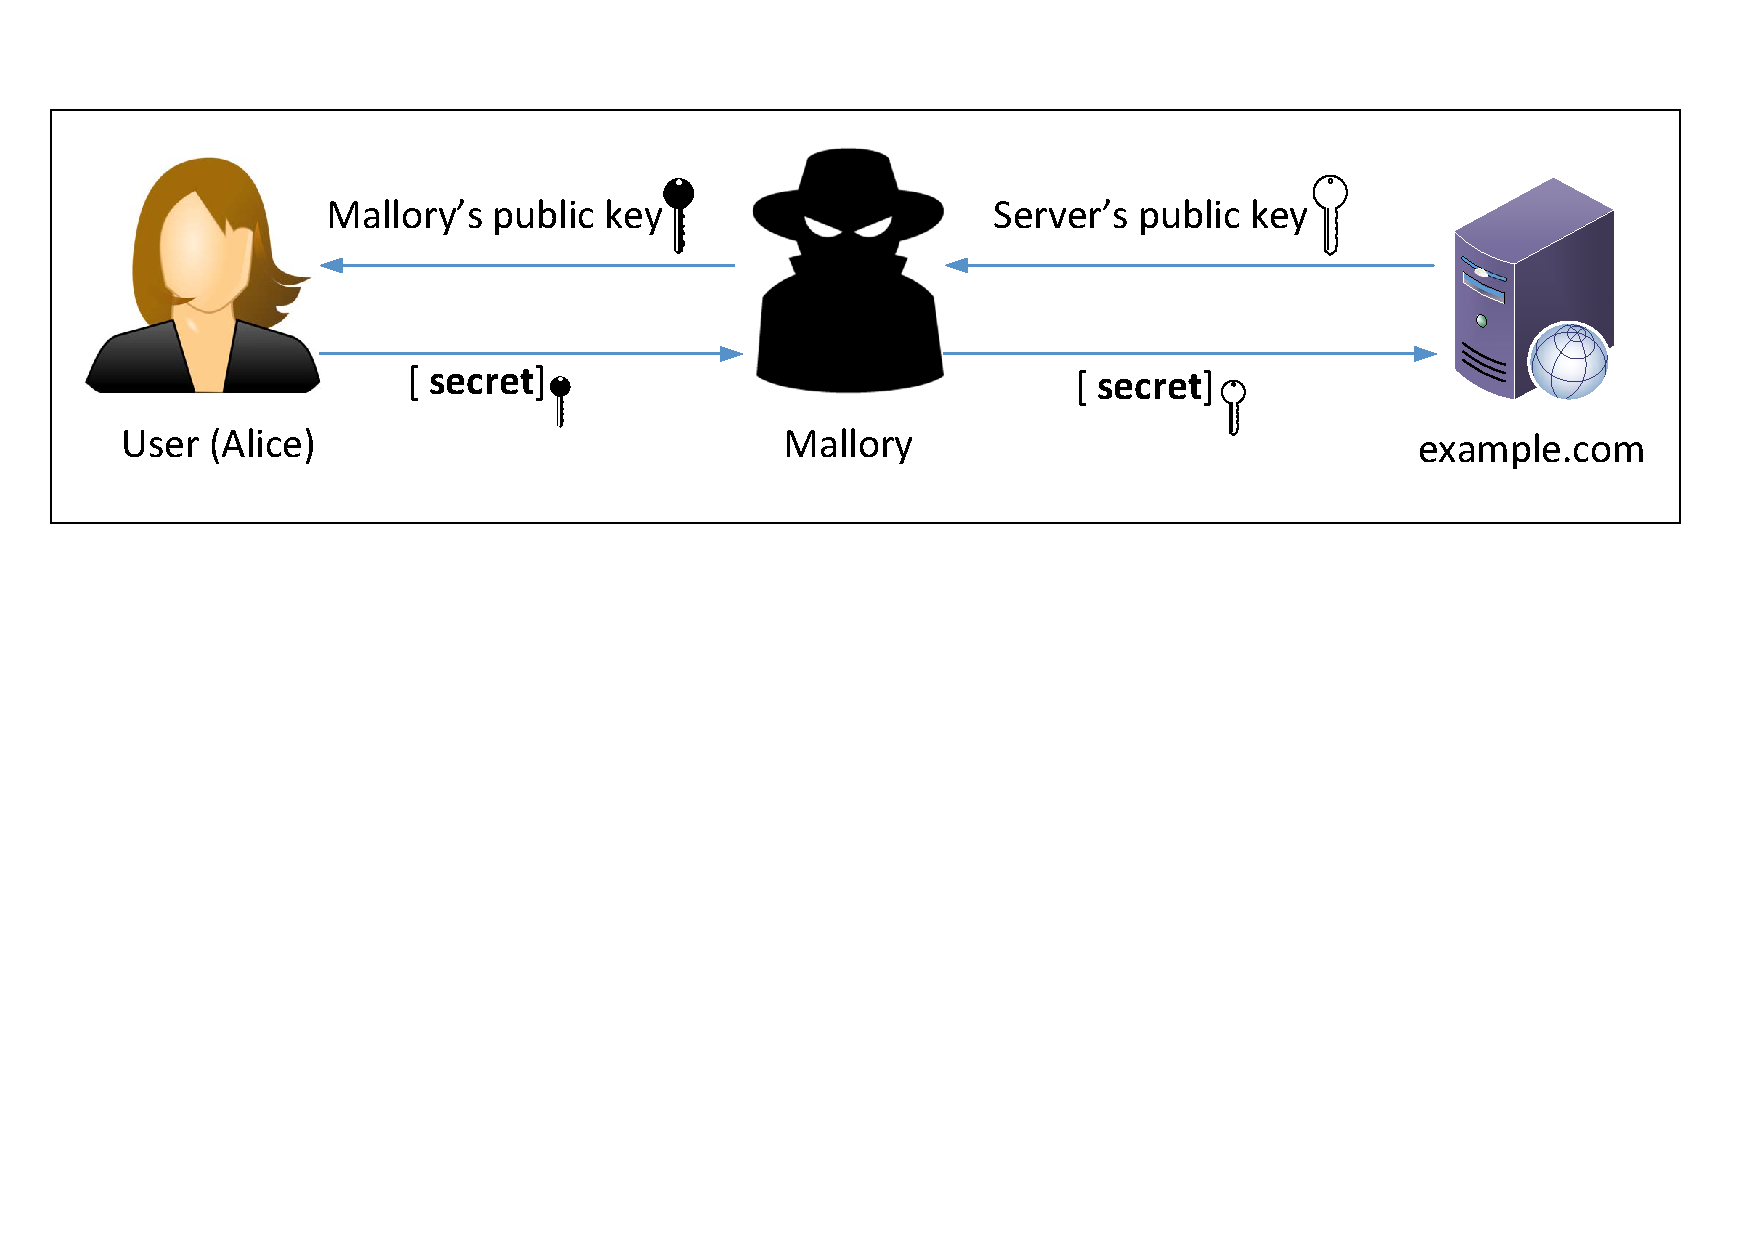
\includegraphics[width=0.8\textwidth]{\pkiFigs/mitm.pdf}
   \end{center}
   \caption{A Man-In-The-Middle (MITM) attack}
   \label{pki:fig:mitm}
\end{figure}



The goal of this task is to help students understand how PKI can defeat such MITM attacks. 
In the task, we will emulate an MITM attack, and see how exactly PKI can defeat it.
We will select a target website first. In this document, we use 
\texttt{www.example.com} as the target website, but in the task, to make it more meaningful,
students should pick a popular website, such as a banking site and social network site. 


\paragraph{Step 1: Setting up the malicious website.} 
In Task 4, we have already set up an HTTPS website. We will
use the same Apache server to impersonate \texttt{www.example.com} (or the site chosen by students).  
To achieve that, we will follow the instruction in Task 4 to 
add a \texttt{VirtualHost} entry to Apache's SSL configuration file: the
\texttt{ServerName} should be \texttt{www.example.com}, but the rest of the
configuration can be the same as that used in Task 4. Obviously, in the real world,
you won't be able to get a valid certificate for \texttt{www.example.com}, 
so we will use the same certificate that we used for our own server. 


Our goal is the following: when a user tries to visit \texttt{www.example.com}, 
we are going to get the user to land in our server, which hosts 
a fake website for \texttt{www.example.com}. If this were a social network
website, The fake site can display a login page similar to the
one in the target website. If users cannot tell the difference, they may type their account credentials
in the fake webpage, essentially disclosing the credentials to the attacker. 


\paragraph{Step 2: Becoming the man in the middle} 
There are several ways to get the user's HTTPS request to land in our web server. One way is to
attack the routing, so the user's HTTPS request is routed to our web server. Another way is
to attack DNS, so when the victim's machine tries to find out the IP address of the target
web server, it gets the IP address of our web server. In this task, we simulate
the attack-DNS approach. Instead of
launching an actual DNS cache poisoning attack, we simply modify the victim's machine's 
\texttt{/etc/hosts} file to emulate the result of a DNS cache positing attack by 
mapping the hostname \texttt{www.example.com} to our malicious web server.


\begin{lstlisting}
10.9.0.80  www.example.com
\end{lstlisting}


\paragraph{Step 3: Browse the target website.}
With everything set up, now visit the target real website, and 
see what your browser would say. Please explain what you have observed. 




% -------------------------------------------
% SUBSECTION
% ------------------------------------------- 
\subsection{Task 6: Launching a Man-In-The-Middle Attack with a Compromised CA}

In this task, we assume that the root CA created in Task 1 is compromised by an attacker, 
and its private key is stolen. Therefore, the attacker can generate any arbitrary certificate 
using this CA's private key. In this task, we will see 
the consequence of such a compromise. 


Please design an experiment to show that the attacker can successfully launch MITM attacks on
any HTTPS website. You can use the same setting created in Task 5, but this time, you need to
demonstrate that the MITM attack is successful, i.e., the browser will not 
raise any suspicion when the victim tries to visit a website but land in the MITM attacker's
fake website.



% *******************************************
% SECTION
% ******************************************* 
\section{Submission}

%%%%%%%%%%%%%%%%%%%%%%%%%%%%%%%%%%%%%%%%

You need to submit a detailed lab report, with screenshots,
to describe what you have done and what you have observed.
You also need to provide explanation
to the observations that are interesting or surprising.
Please also list the important code snippets followed by
explanation. Simply attaching code without any explanation will not
receive credits.

%%%%%%%%%%%%%%%%%%%%%%%%%%%%%%%%%%%%%%%%


%%%%%%%%%%%%%%%%%%%%%%%%%%%%%%%%%%%%%%%%%%%%%%%%%%%%%%
\end{document}
%%%%%%%%%%%%%%%%%%%%%%%%%%%%%%%%%%%%%%%%%%%%%%%%%%%%%%

